
\documentclass{article} % For LaTeX2e
\usepackage{iclr2025_conference,times}

% Optional math commands from https://github.com/goodfeli/dlbook_notation.
%%%%% NEW MATH DEFINITIONS %%%%%

\usepackage{amsmath,amsfonts,bm}

% Mark sections of captions for referring to divisions of figures
\newcommand{\figleft}{{\em (Left)}}
\newcommand{\figcenter}{{\em (Center)}}
\newcommand{\figright}{{\em (Right)}}
\newcommand{\figtop}{{\em (Top)}}
\newcommand{\figbottom}{{\em (Bottom)}}
\newcommand{\captiona}{{\em (a)}}
\newcommand{\captionb}{{\em (b)}}
\newcommand{\captionc}{{\em (c)}}
\newcommand{\captiond}{{\em (d)}}

% Highlight a newly defined term
\newcommand{\newterm}[1]{{\bf #1}}


% Figure reference, lower-case.
\def\figref#1{figure~\ref{#1}}
% Figure reference, capital. For start of sentence
\def\Figref#1{Figure~\ref{#1}}
\def\twofigref#1#2{figures \ref{#1} and \ref{#2}}
\def\quadfigref#1#2#3#4{figures \ref{#1}, \ref{#2}, \ref{#3} and \ref{#4}}
% Section reference, lower-case.
\def\secref#1{section~\ref{#1}}
% Section reference, capital.
\def\Secref#1{Section~\ref{#1}}
% Reference to two sections.
\def\twosecrefs#1#2{sections \ref{#1} and \ref{#2}}
% Reference to three sections.
\def\secrefs#1#2#3{sections \ref{#1}, \ref{#2} and \ref{#3}}
% Reference to an equation, lower-case.
\def\eqref#1{equation~\ref{#1}}
% Reference to an equation, upper case
\def\Eqref#1{Equation~\ref{#1}}
% A raw reference to an equation---avoid using if possible
\def\plaineqref#1{\ref{#1}}
% Reference to a chapter, lower-case.
\def\chapref#1{chapter~\ref{#1}}
% Reference to an equation, upper case.
\def\Chapref#1{Chapter~\ref{#1}}
% Reference to a range of chapters
\def\rangechapref#1#2{chapters\ref{#1}--\ref{#2}}
% Reference to an algorithm, lower-case.
\def\algref#1{algorithm~\ref{#1}}
% Reference to an algorithm, upper case.
\def\Algref#1{Algorithm~\ref{#1}}
\def\twoalgref#1#2{algorithms \ref{#1} and \ref{#2}}
\def\Twoalgref#1#2{Algorithms \ref{#1} and \ref{#2}}
% Reference to a part, lower case
\def\partref#1{part~\ref{#1}}
% Reference to a part, upper case
\def\Partref#1{Part~\ref{#1}}
\def\twopartref#1#2{parts \ref{#1} and \ref{#2}}

\def\ceil#1{\lceil #1 \rceil}
\def\floor#1{\lfloor #1 \rfloor}
\def\1{\bm{1}}
\newcommand{\train}{\mathcal{D}}
\newcommand{\valid}{\mathcal{D_{\mathrm{valid}}}}
\newcommand{\test}{\mathcal{D_{\mathrm{test}}}}

\def\eps{{\epsilon}}


% Random variables
\def\reta{{\textnormal{$\eta$}}}
\def\ra{{\textnormal{a}}}
\def\rb{{\textnormal{b}}}
\def\rc{{\textnormal{c}}}
\def\rd{{\textnormal{d}}}
\def\re{{\textnormal{e}}}
\def\rf{{\textnormal{f}}}
\def\rg{{\textnormal{g}}}
\def\rh{{\textnormal{h}}}
\def\ri{{\textnormal{i}}}
\def\rj{{\textnormal{j}}}
\def\rk{{\textnormal{k}}}
\def\rl{{\textnormal{l}}}
% rm is already a command, just don't name any random variables m
\def\rn{{\textnormal{n}}}
\def\ro{{\textnormal{o}}}
\def\rp{{\textnormal{p}}}
\def\rq{{\textnormal{q}}}
\def\rr{{\textnormal{r}}}
\def\rs{{\textnormal{s}}}
\def\rt{{\textnormal{t}}}
\def\ru{{\textnormal{u}}}
\def\rv{{\textnormal{v}}}
\def\rw{{\textnormal{w}}}
\def\rx{{\textnormal{x}}}
\def\ry{{\textnormal{y}}}
\def\rz{{\textnormal{z}}}

% Random vectors
\def\rvepsilon{{\mathbf{\epsilon}}}
\def\rvtheta{{\mathbf{\theta}}}
\def\rva{{\mathbf{a}}}
\def\rvb{{\mathbf{b}}}
\def\rvc{{\mathbf{c}}}
\def\rvd{{\mathbf{d}}}
\def\rve{{\mathbf{e}}}
\def\rvf{{\mathbf{f}}}
\def\rvg{{\mathbf{g}}}
\def\rvh{{\mathbf{h}}}
\def\rvu{{\mathbf{i}}}
\def\rvj{{\mathbf{j}}}
\def\rvk{{\mathbf{k}}}
\def\rvl{{\mathbf{l}}}
\def\rvm{{\mathbf{m}}}
\def\rvn{{\mathbf{n}}}
\def\rvo{{\mathbf{o}}}
\def\rvp{{\mathbf{p}}}
\def\rvq{{\mathbf{q}}}
\def\rvr{{\mathbf{r}}}
\def\rvs{{\mathbf{s}}}
\def\rvt{{\mathbf{t}}}
\def\rvu{{\mathbf{u}}}
\def\rvv{{\mathbf{v}}}
\def\rvw{{\mathbf{w}}}
\def\rvx{{\mathbf{x}}}
\def\rvy{{\mathbf{y}}}
\def\rvz{{\mathbf{z}}}

% Elements of random vectors
\def\erva{{\textnormal{a}}}
\def\ervb{{\textnormal{b}}}
\def\ervc{{\textnormal{c}}}
\def\ervd{{\textnormal{d}}}
\def\erve{{\textnormal{e}}}
\def\ervf{{\textnormal{f}}}
\def\ervg{{\textnormal{g}}}
\def\ervh{{\textnormal{h}}}
\def\ervi{{\textnormal{i}}}
\def\ervj{{\textnormal{j}}}
\def\ervk{{\textnormal{k}}}
\def\ervl{{\textnormal{l}}}
\def\ervm{{\textnormal{m}}}
\def\ervn{{\textnormal{n}}}
\def\ervo{{\textnormal{o}}}
\def\ervp{{\textnormal{p}}}
\def\ervq{{\textnormal{q}}}
\def\ervr{{\textnormal{r}}}
\def\ervs{{\textnormal{s}}}
\def\ervt{{\textnormal{t}}}
\def\ervu{{\textnormal{u}}}
\def\ervv{{\textnormal{v}}}
\def\ervw{{\textnormal{w}}}
\def\ervx{{\textnormal{x}}}
\def\ervy{{\textnormal{y}}}
\def\ervz{{\textnormal{z}}}

% Random matrices
\def\rmA{{\mathbf{A}}}
\def\rmB{{\mathbf{B}}}
\def\rmC{{\mathbf{C}}}
\def\rmD{{\mathbf{D}}}
\def\rmE{{\mathbf{E}}}
\def\rmF{{\mathbf{F}}}
\def\rmG{{\mathbf{G}}}
\def\rmH{{\mathbf{H}}}
\def\rmI{{\mathbf{I}}}
\def\rmJ{{\mathbf{J}}}
\def\rmK{{\mathbf{K}}}
\def\rmL{{\mathbf{L}}}
\def\rmM{{\mathbf{M}}}
\def\rmN{{\mathbf{N}}}
\def\rmO{{\mathbf{O}}}
\def\rmP{{\mathbf{P}}}
\def\rmQ{{\mathbf{Q}}}
\def\rmR{{\mathbf{R}}}
\def\rmS{{\mathbf{S}}}
\def\rmT{{\mathbf{T}}}
\def\rmU{{\mathbf{U}}}
\def\rmV{{\mathbf{V}}}
\def\rmW{{\mathbf{W}}}
\def\rmX{{\mathbf{X}}}
\def\rmY{{\mathbf{Y}}}
\def\rmZ{{\mathbf{Z}}}

% Elements of random matrices
\def\ermA{{\textnormal{A}}}
\def\ermB{{\textnormal{B}}}
\def\ermC{{\textnormal{C}}}
\def\ermD{{\textnormal{D}}}
\def\ermE{{\textnormal{E}}}
\def\ermF{{\textnormal{F}}}
\def\ermG{{\textnormal{G}}}
\def\ermH{{\textnormal{H}}}
\def\ermI{{\textnormal{I}}}
\def\ermJ{{\textnormal{J}}}
\def\ermK{{\textnormal{K}}}
\def\ermL{{\textnormal{L}}}
\def\ermM{{\textnormal{M}}}
\def\ermN{{\textnormal{N}}}
\def\ermO{{\textnormal{O}}}
\def\ermP{{\textnormal{P}}}
\def\ermQ{{\textnormal{Q}}}
\def\ermR{{\textnormal{R}}}
\def\ermS{{\textnormal{S}}}
\def\ermT{{\textnormal{T}}}
\def\ermU{{\textnormal{U}}}
\def\ermV{{\textnormal{V}}}
\def\ermW{{\textnormal{W}}}
\def\ermX{{\textnormal{X}}}
\def\ermY{{\textnormal{Y}}}
\def\ermZ{{\textnormal{Z}}}

% Vectors
\def\vzero{{\bm{0}}}
\def\vone{{\bm{1}}}
\def\vmu{{\bm{\mu}}}
\def\vtheta{{\bm{\theta}}}
\def\va{{\bm{a}}}
\def\vb{{\bm{b}}}
\def\vc{{\bm{c}}}
\def\vd{{\bm{d}}}
\def\ve{{\bm{e}}}
\def\vf{{\bm{f}}}
\def\vg{{\bm{g}}}
\def\vh{{\bm{h}}}
\def\vi{{\bm{i}}}
\def\vj{{\bm{j}}}
\def\vk{{\bm{k}}}
\def\vl{{\bm{l}}}
\def\vm{{\bm{m}}}
\def\vn{{\bm{n}}}
\def\vo{{\bm{o}}}
\def\vp{{\bm{p}}}
\def\vq{{\bm{q}}}
\def\vr{{\bm{r}}}
\def\vs{{\bm{s}}}
\def\vt{{\bm{t}}}
\def\vu{{\bm{u}}}
\def\vv{{\bm{v}}}
\def\vw{{\bm{w}}}
\def\vx{{\bm{x}}}
\def\vy{{\bm{y}}}
\def\vz{{\bm{z}}}

% Elements of vectors
\def\evalpha{{\alpha}}
\def\evbeta{{\beta}}
\def\evepsilon{{\epsilon}}
\def\evlambda{{\lambda}}
\def\evomega{{\omega}}
\def\evmu{{\mu}}
\def\evpsi{{\psi}}
\def\evsigma{{\sigma}}
\def\evtheta{{\theta}}
\def\eva{{a}}
\def\evb{{b}}
\def\evc{{c}}
\def\evd{{d}}
\def\eve{{e}}
\def\evf{{f}}
\def\evg{{g}}
\def\evh{{h}}
\def\evi{{i}}
\def\evj{{j}}
\def\evk{{k}}
\def\evl{{l}}
\def\evm{{m}}
\def\evn{{n}}
\def\evo{{o}}
\def\evp{{p}}
\def\evq{{q}}
\def\evr{{r}}
\def\evs{{s}}
\def\evt{{t}}
\def\evu{{u}}
\def\evv{{v}}
\def\evw{{w}}
\def\evx{{x}}
\def\evy{{y}}
\def\evz{{z}}

% Matrix
\def\mA{{\bm{A}}}
\def\mB{{\bm{B}}}
\def\mC{{\bm{C}}}
\def\mD{{\bm{D}}}
\def\mE{{\bm{E}}}
\def\mF{{\bm{F}}}
\def\mG{{\bm{G}}}
\def\mH{{\bm{H}}}
\def\mI{{\bm{I}}}
\def\mJ{{\bm{J}}}
\def\mK{{\bm{K}}}
\def\mL{{\bm{L}}}
\def\mM{{\bm{M}}}
\def\mN{{\bm{N}}}
\def\mO{{\bm{O}}}
\def\mP{{\bm{P}}}
\def\mQ{{\bm{Q}}}
\def\mR{{\bm{R}}}
\def\mS{{\bm{S}}}
\def\mT{{\bm{T}}}
\def\mU{{\bm{U}}}
\def\mV{{\bm{V}}}
\def\mW{{\bm{W}}}
\def\mX{{\bm{X}}}
\def\mY{{\bm{Y}}}
\def\mZ{{\bm{Z}}}
\def\mBeta{{\bm{\beta}}}
\def\mPhi{{\bm{\Phi}}}
\def\mLambda{{\bm{\Lambda}}}
\def\mSigma{{\bm{\Sigma}}}

% Tensor
\DeclareMathAlphabet{\mathsfit}{\encodingdefault}{\sfdefault}{m}{sl}
\SetMathAlphabet{\mathsfit}{bold}{\encodingdefault}{\sfdefault}{bx}{n}
\newcommand{\tens}[1]{\bm{\mathsfit{#1}}}
\def\tA{{\tens{A}}}
\def\tB{{\tens{B}}}
\def\tC{{\tens{C}}}
\def\tD{{\tens{D}}}
\def\tE{{\tens{E}}}
\def\tF{{\tens{F}}}
\def\tG{{\tens{G}}}
\def\tH{{\tens{H}}}
\def\tI{{\tens{I}}}
\def\tJ{{\tens{J}}}
\def\tK{{\tens{K}}}
\def\tL{{\tens{L}}}
\def\tM{{\tens{M}}}
\def\tN{{\tens{N}}}
\def\tO{{\tens{O}}}
\def\tP{{\tens{P}}}
\def\tQ{{\tens{Q}}}
\def\tR{{\tens{R}}}
\def\tS{{\tens{S}}}
\def\tT{{\tens{T}}}
\def\tU{{\tens{U}}}
\def\tV{{\tens{V}}}
\def\tW{{\tens{W}}}
\def\tX{{\tens{X}}}
\def\tY{{\tens{Y}}}
\def\tZ{{\tens{Z}}}


% Graph
\def\gA{{\mathcal{A}}}
\def\gB{{\mathcal{B}}}
\def\gC{{\mathcal{C}}}
\def\gD{{\mathcal{D}}}
\def\gE{{\mathcal{E}}}
\def\gF{{\mathcal{F}}}
\def\gG{{\mathcal{G}}}
\def\gH{{\mathcal{H}}}
\def\gI{{\mathcal{I}}}
\def\gJ{{\mathcal{J}}}
\def\gK{{\mathcal{K}}}
\def\gL{{\mathcal{L}}}
\def\gM{{\mathcal{M}}}
\def\gN{{\mathcal{N}}}
\def\gO{{\mathcal{O}}}
\def\gP{{\mathcal{P}}}
\def\gQ{{\mathcal{Q}}}
\def\gR{{\mathcal{R}}}
\def\gS{{\mathcal{S}}}
\def\gT{{\mathcal{T}}}
\def\gU{{\mathcal{U}}}
\def\gV{{\mathcal{V}}}
\def\gW{{\mathcal{W}}}
\def\gX{{\mathcal{X}}}
\def\gY{{\mathcal{Y}}}
\def\gZ{{\mathcal{Z}}}

% Sets
\def\sA{{\mathbb{A}}}
\def\sB{{\mathbb{B}}}
\def\sC{{\mathbb{C}}}
\def\sD{{\mathbb{D}}}
% Don't use a set called E, because this would be the same as our symbol
% for expectation.
\def\sF{{\mathbb{F}}}
\def\sG{{\mathbb{G}}}
\def\sH{{\mathbb{H}}}
\def\sI{{\mathbb{I}}}
\def\sJ{{\mathbb{J}}}
\def\sK{{\mathbb{K}}}
\def\sL{{\mathbb{L}}}
\def\sM{{\mathbb{M}}}
\def\sN{{\mathbb{N}}}
\def\sO{{\mathbb{O}}}
\def\sP{{\mathbb{P}}}
\def\sQ{{\mathbb{Q}}}
\def\sR{{\mathbb{R}}}
\def\sS{{\mathbb{S}}}
\def\sT{{\mathbb{T}}}
\def\sU{{\mathbb{U}}}
\def\sV{{\mathbb{V}}}
\def\sW{{\mathbb{W}}}
\def\sX{{\mathbb{X}}}
\def\sY{{\mathbb{Y}}}
\def\sZ{{\mathbb{Z}}}

% Entries of a matrix
\def\emLambda{{\Lambda}}
\def\emA{{A}}
\def\emB{{B}}
\def\emC{{C}}
\def\emD{{D}}
\def\emE{{E}}
\def\emF{{F}}
\def\emG{{G}}
\def\emH{{H}}
\def\emI{{I}}
\def\emJ{{J}}
\def\emK{{K}}
\def\emL{{L}}
\def\emM{{M}}
\def\emN{{N}}
\def\emO{{O}}
\def\emP{{P}}
\def\emQ{{Q}}
\def\emR{{R}}
\def\emS{{S}}
\def\emT{{T}}
\def\emU{{U}}
\def\emV{{V}}
\def\emW{{W}}
\def\emX{{X}}
\def\emY{{Y}}
\def\emZ{{Z}}
\def\emSigma{{\Sigma}}

% entries of a tensor
% Same font as tensor, without \bm wrapper
\newcommand{\etens}[1]{\mathsfit{#1}}
\def\etLambda{{\etens{\Lambda}}}
\def\etA{{\etens{A}}}
\def\etB{{\etens{B}}}
\def\etC{{\etens{C}}}
\def\etD{{\etens{D}}}
\def\etE{{\etens{E}}}
\def\etF{{\etens{F}}}
\def\etG{{\etens{G}}}
\def\etH{{\etens{H}}}
\def\etI{{\etens{I}}}
\def\etJ{{\etens{J}}}
\def\etK{{\etens{K}}}
\def\etL{{\etens{L}}}
\def\etM{{\etens{M}}}
\def\etN{{\etens{N}}}
\def\etO{{\etens{O}}}
\def\etP{{\etens{P}}}
\def\etQ{{\etens{Q}}}
\def\etR{{\etens{R}}}
\def\etS{{\etens{S}}}
\def\etT{{\etens{T}}}
\def\etU{{\etens{U}}}
\def\etV{{\etens{V}}}
\def\etW{{\etens{W}}}
\def\etX{{\etens{X}}}
\def\etY{{\etens{Y}}}
\def\etZ{{\etens{Z}}}

% The true underlying data generating distribution
\newcommand{\pdata}{p_{\rm{data}}}
% The empirical distribution defined by the training set
\newcommand{\ptrain}{\hat{p}_{\rm{data}}}
\newcommand{\Ptrain}{\hat{P}_{\rm{data}}}
% The model distribution
\newcommand{\pmodel}{p_{\rm{model}}}
\newcommand{\Pmodel}{P_{\rm{model}}}
\newcommand{\ptildemodel}{\tilde{p}_{\rm{model}}}
% Stochastic autoencoder distributions
\newcommand{\pencode}{p_{\rm{encoder}}}
\newcommand{\pdecode}{p_{\rm{decoder}}}
\newcommand{\precons}{p_{\rm{reconstruct}}}

\newcommand{\laplace}{\mathrm{Laplace}} % Laplace distribution

\newcommand{\E}{\mathbb{E}}
\newcommand{\Ls}{\mathcal{L}}
\newcommand{\R}{\mathbb{R}}
\newcommand{\emp}{\tilde{p}}
\newcommand{\lr}{\alpha}
\newcommand{\reg}{\lambda}
\newcommand{\rect}{\mathrm{rectifier}}
\newcommand{\softmax}{\mathrm{softmax}}
\newcommand{\sigmoid}{\sigma}
\newcommand{\softplus}{\zeta}
\newcommand{\KL}{D_{\mathrm{KL}}}
\newcommand{\Var}{\mathrm{Var}}
\newcommand{\standarderror}{\mathrm{SE}}
\newcommand{\Cov}{\mathrm{Cov}}
% Wolfram Mathworld says $L^2$ is for function spaces and $\ell^2$ is for vectors
% But then they seem to use $L^2$ for vectors throughout the site, and so does
% wikipedia.
\newcommand{\normlzero}{L^0}
\newcommand{\normlone}{L^1}
\newcommand{\normltwo}{L^2}
\newcommand{\normlp}{L^p}
\newcommand{\normmax}{L^\infty}

\newcommand{\parents}{Pa} % See usage in notation.tex. Chosen to match Daphne's book.

\DeclareMathOperator*{\argmax}{arg\,max}
\DeclareMathOperator*{\argmin}{arg\,min}

\DeclareMathOperator{\sign}{sign}
\DeclareMathOperator{\Tr}{Tr}
\let\ab\allowbreak


\usepackage{hyperref}
\usepackage{url}
\usepackage{graphicx} % For including images
\usepackage{booktabs} % For professional-looking tables


\title{INF8245E Fall2024  \\ Kaggle competition \\ Team\_1 }

% Authors must not appear in the submitted version. They should be hidden
% as long as the \iclrfinalcopy macro remains commented out below.
% Non-anonymous submissions will be rejected without review.

\author{Alexis Nicolas - 2143258 \\
\texttt{\ alexis.nicolas@polymtl.ca} \\
\And
Sidney Gharib - 2145565 \\
\texttt{\ sidney.gharib@polymtl.ca} \\
\And
Elizabeth Michaud - 2073093 \\
\texttt{\ elizabeth-1.michaud@polymtl.ca} \\
}

% The \author macro works with any number of authors. There are two commands
% used to separate the names and addresses of multiple authors: \And and \AND.
%
% Using \And between authors leaves it to \LaTeX{} to determine where to break
% the lines. Using \AND forces a linebreak at that point. So, if \LaTeX{}
% puts 3 of 4 authors names on the first line, and the last on the second
% line, try using \AND instead of \And before the third author name.

\newcommand{\fix}{\marginpar{FIX}}
\newcommand{\new}{\marginpar{NEW}}

\iclrfinalcopy % Uncomment for camera-ready version, but NOT for submission.
\begin{document}


\maketitle

\begin{abstract}
This Kaggle explores the relationship between lifestyle factors and the likelihood of diabetes diagnosis.
Utilizing a dataset of 200,000 records with 28 features encompassing demographics,
laboratory test results, and survey responses, we aim to construct predictive models that can identify whether an individual has diabetes.
The research leverages machine learning methodologies to uncover significant patterns and provide actionable insights into the interplay between lifestyle and diabetes risk.
\end{abstract}

\section{Feature design}

The first step was to explore the dataset to understand the kind of data and features we were working with. By doing so, we were 
able to notice that the dataset had more than 200,000 samples and 28 features. While most of the features were numerical 
(binary, discrete and continuous numbers), a few of them were of type "object". 

For each of the discrete and continuous number features, we made a boxplot of their values in the dataset and displayed it. 
This helped us visualize the distribution of the numerical features and their outliers values. The features BMI, MentHlth and PhysHlth
are the features for which there is the most outliers. This is an information the we had to keep in mind while developing our models.

For each of the binary features, we made a plot that showed the distribution of "yes" and "no" labels per possible values which are 0 and 1 since they are binary features. 
When the percentage of "yes" is very similar for 0 and 1, it could mean that the feature in question doesn't have a significant 
impact on the label. Therefore, we considered removing that feature from the model training. 

Since we also wished to explore the features that were non-numerical, we used an ordinal encoding for the features BMI Category, 
Age Group, Education Level and Income Group. We used scikit-learn OrdinalEncoder. Because these features can only take a small amount of different values, we were able to 
specify the order of importance between the different values. For instance, the only possible values for Income Group are "Low Income", 
"Middle Income" and "High Income". It is simple to determine that Low Income is inferior to Middle Income which is inferior to High 
Income. It is important to specify the order, otherwise the ordinal encoder will encode the values in alphabetical order.

Once all the features were encoded, we were able to plot a graph representing the correlation between Diabetes binary 
values from labels.csv and each of the features. We used pandas.DataFrame.corrwith function in order to make such graph. 
The resulting graph shows how much each 28 features tend to affect the diabetes diagnosis. When the result for a feature is positive, 
it means that samples that have a higher value for this feature tends to be labelled as "yes" and vice versa. If the result for a 
feature was very close to zero, we considered removing that feature from the training step. 

We used another metric, called the mutual information score, to measure how much each feature impacts the diagnosis. We computed the mutual 
information score separately for the binary features, the continuous numerical features and the discrete numerical features. 
The lower is the score, the lower should be the impact that this feature has on the diagnosis. This metric was also considered when 
trying to make a good feature selection.

Next, we tried to used the normal probability plot of the features to verify if they were following a Gaussian distribution. It was not 
the case, but if it had been the case, we could potentially have obtained a good classifier by using a Gaussian Naive Bayes model.

Finally, the last method we used in order to select the features to keep was the correlation matrix. By using a correlation matrix, we 
were able to notice if some of the features were highly correlated. If two features are highly correlated, it might not be useful to 
keep both of them to train the model. 

After taking into consideration all of the metrics, we were able to filter out some features from the training step. We decided to 
remove Age Group, MentHlth, HvyAlcoholConsump, NoDocbcCost, Smoker, Fruits, Veggies, Mental Health Risk and AnyHealthcare. 
We tried another combinations of features to remove, but we noticed that this feature selection was the one that gave the best results.
Other features were removed for models where we used PCA. 

In order to complete the data preprocessing, we encoded all the non-numerical features using scikit-learn LabelEncoder, we split the 
dataset into a training set and a validation set and we normalized the training set, the validation set and the testing set using 
scikit-learn StandartScaler. 


\section{Algorithms}

Since we wanted to increase our chances of obtaining a higher score in the Kaggle competition, we trained many different models. We will 
briefly explain the algorithm behind our 5 best models.

Firstly, we used a Random Forest model which is an ensemble learning method that uses multiple decision trees to produce an output. 
It allows to make a better generalization than a single decision tree alone. In order to train all the different decision trees, 
the Random Forest creates a subset of the training set for each decision tree. When we want to make a prediction, each decision tree will 
give its own prediction value and the Random Forest will use the most common prediction value among the decision trees as its prediction value.

Secondly, we used a Decision Tree model with Adaboosting. First of all, a Decision Tree is a model that tries to leaning decision rules from the 
features of the training set. It starts from a root node from where the training set will be split into branches accordingly to the decision rules 
represented by the internal nodes. The leaves of the decision tree represent the class label the tree is going to predict if a sample followed all 
the branches down to that leaf node. Then, we used Adaboosting, an ensemble learning method, on top of our decision tree model. This algorithm trains 
multiple weak learners sequentially, decision stumps in the case of a Decision Tree model, while focussing on the samples that were misclassified. 
Samples that were misclassified will have a more important weight when training the next weak learner. The prediction of this model is given by a 
weighted combination of all learners prediction.

Thirdly, we used a Logistic Regression model which is a probabilistic discriminative model. With the discriminative approach, we want to learn the 
model's parameters directly from the maximum likelihood. The Logistic Regression classifier models the probability of a class by mapping the linear 
combination of the input features with a sigmoid function. For a 2-class classifier, the predicted value is between 0 and 1. If it's greater or equal 
to 0.5, it means the model predicted the positive class for the given sample. Otherwise, the model predicted the negative class. 

Fourthly, we used a Logistic Regression model with Adaboosting. The idea is very similar to Adaboosting with a Decision Tree model, but instead of 
using decision stumps as weak learners, we use a simpler version of a logistic regression.

Fifthly, we used a Neural Network. This model is formed by multiple layers such as an input layer followed by hidden layers that each has its activation 
layer. The last layer is an output layer. Layers have multiple neurons and every neurons make a computation on an input and pass the result to the next 
layer. This is called the forward pass. After, the Neural Network executes a backward pass during which it updates the weights for each neurons. The 
goal is to minimize the error score using gradient descent. 


\section{Methodology}
\label{headings}


\subsection{Training-Validation split}

We decided to split our training set into a training and validation set with a ratio of 90\% and 10\% respectively,
because we considered that 202944 samples was enough so that only 10\%(20294 samples) would give us a good approximation of the
accuracies of our models.

The validation would be used to measure the performances during training,
telling us which hyperparameters gives the bests results, and telling us where
to stop tne training to avoid overfitting.

We made sure to shuffle the set to avoid data that would be ordered, and we used a stratified split to make sure
the validation and training set would have the same proportion of positive and negative samples.

\subsection{normal distribution of the features}
We looked at the normal probability plot for each of the features to find if they were disctributed
according to a normal distribution. Except for the age feature, all of them where not distributed
like a gaussian dstribution. Furthermore, many of the features were binary instead of continuous.

Because of the lack of featutres with a normal distribution and many important features being binary or classes,
we decided it would not be worth to try to do a naive bayes classifier.

\subsection{Optimisation for the deep neural network}
We used cuda cores to train our deep neural network model with the Pytorch library.
This made the training of a neural network way faster than if we have kept the training set on the cpu.
With this optimisation we were able to quickly test different configurations for the hidden layers,
like the number of neurons and the number of hidden layers.
We also tested different activation fonctions like the ReLU and the Leaky ReLU.
We tested different optimisers like the ADAM and SGD.
We used the binary classification error to measure the loss of the model,
with a weight added to the class 1, since the dataset was imbalenced with fewer positives samples.
We tried to train the model using mini-batch gradient descent and full batch gradient.
Finally, we used the validation set to stop the training when the F1-score of its predictions was not improving anymore.


Unfortunately, all of the combinations of theses models, loss functions, activation functions, optimisers and epoch of training were not able to produce
better results than our other models. All of the neural networks we tried seemed to give us the same F1-score on the validation set.

Since the models always predicted true positive at around 50\%, we tried tweaking the value of the treshold
of the prediction to further improve the accuracy on the class 1. Even though lowering it down to 0.1 gave us a small improvement,
it was not significant enough to make a change, since the number of false negatives also augmented and the recall dropped.


\subsection{finding the optimal hyperparameters for the models}
We also tried other models seen in class. For theses, we used the sklearn library to train them and find
the best hyperparamaters. We used a grid search algorithm to find the best combination of hyperparameters
for each model. We used the F1-score as a metric for the grid search, since it was the one we wanted to maximise.
Since the training and evalluation of each combination of hyperparameter is a very long. We used a gave a few hyperparameter
set to the grid search. 



\section{Results}
The results from table \ref{tab:validation-F1-scores} are the models validation F1-scores reveal important insights into their performance on the classification task. Among all tested models, the custom Neural Network achieved the highest validation F1-score of 0.4706, demonstrating its effectiveness at capturing complex patterns in the data. This superior performance can be attributed to the carefully designed architecture, which includes multiple layers with dropout regularization, Xavier initialization, and the use of leaky ReLU activations. These design choices appear to enhance the network's ability to generalize, making it the most effective model in this comparison.

The Logistic Regression model, with a validation F1-score of 0.4620, emerged as the second-best performer. Its strong result highlights the model's simplicity and robustness for binary classification tasks. Interestingly, Logistic Regression outperformed ensemble techniques like Adaboosting, which scored slightly lower at 0.4582. This outcome suggests that while boosting often improves base model performance, it may not provide significant gains for Logistic Regression in this dataset.

Random Forest models also performed well, with the standalone Random Forest achieving a validation F1-score of 0.4589. This model's ensemble nature likely helped capture the nuances of the dataset. However, when dimensionality reduction via PCA was applied, the performance dropped to 0.4309. This decline indicates that PCA may have eliminated features essential for classification, reducing the model's effectiveness. Additionally, Decision Tree models, which serve as a base for Random Forest, showed varied results. The single Decision Tree achieved a validation F1-score of 0.4252, which improved modestly with Bagging to 0.4363 and more significantly with Adaboosting to 0.4588. These results illustrate how ensemble techniques help mitigate the inherent overfitting tendencies of decision trees.

On the other hand, some models struggled to achieve competitive performance. For example, the XGBClassifier's validation F1-score of 0.2949 was surprisingly low, given its reputation as a high-performing algorithm. This outcome may indicate that the model requires further hyperparameter tuning or better feature engineering to suit this dataset. Similarly, K-Nearest Neighbors (KNN) scored only 0.2543, likely due to its inability to handle high-dimensional data effectively without feature selection or dimensionality reduction. The Multilayer Perceptron (MLP) model also underperformed, achieving a validation F1-score of 0.2773, suggesting that it may lack the architectural sophistication or training optimizations present in the custom Neural Network.

The Support Vector Machine (SVM), with a validation F1-score of 0.4357, performed comparably to ensemble models like Decision Tree Bagging. This performance reflects the SVM's ability to model nonlinear relationships in the data, though it fell short of the highest-performing methods.

Overall, the results highlight the advantages of more advanced models like Neural Networks while also showcasing the reliability of simpler models such as Logistic Regression and Random Forest. The modest gains achieved by boosting methods indicate that ensemble techniques are valuable but may require careful tuning to unlock their full potential. Future work could explore additional optimizations, such as hyperparameter tuning for XGBClassifier, further experimentation with Neural Network architectures, and the use of ensemble methods that combine predictions from the strongest individual models. 


In Table \ref{tab:kaggle-scores}, we observe a trend in the public scores of our submissions. From Submission 11 to Submission 6, there is a steady increase in scores, reflecting gradual improvements in our models. Submission 6 achieved the highest score of 0.464, closely followed by Submission 7 with 0.462. Submissions 4 and 5, however, represent experiments involving significant changes to the code, such as altering the distribution and composition of the training and validation sets. Specifically, we attempted to train the models using balanced datasets, ensuring equal representation of the classes. However, this approach did not yield positive results, as the test set's composition was fundamentally different. This highlights the challenge of aligning training strategies with the real-world characteristics of the test data.

The architecture and hyperparameters of the custom neural network in Table \ref{tab:custom-nn-architecture} were designed to address a binary classification problem. The model has 10 hidden layers, starting with 512 units in the initial layers and gradually reducing to 16 units in the final hidden layer. This progression allows the network to learn complex patterns while focusing on essential features as it moves deeper. The Leaky ReLU activation function was used to avoid vanishing gradients and handle negative values, ensuring smoother optimization.

A dropout rate of 0.1 was applied after each layer to reduce overfitting by randomly deactivating neurons during training. The Xavier uniform initialization was chosen to distribute weights optimally at the start, helping stabilize gradient flows through the network. The output layer consists of a single unit for binary classification, with BCEWithLogitsLoss as the loss function. This was combined with a positive class weighting factor to handle imbalances in the dataset.

The NAdam optimizer was used for training, combining the benefits of Adam optimization and Nesterov momentum. A learning rate of 0.005 was set to balance the speed of convergence and training stability. The model was trained over 100 epochs, providing enough time to learn the data's patterns without overfitting.


Figure \ref{tab:validation-F1-scores} shows the training and validation loss, as well as the F1-score over 100 epochs. There is a gradual decrease in the training loss until around 30 epochs. The validation loss, on the other hand, remains stable throughout most of the training, with a plateau in the error between epochs 10 and 20. The F1-score consistently stays between 0.40 and 0.47. Therefore, it may be possible to reduce the number of epochs since all metrics converge starting from around 70 epochs.


\section{Discussion}

Our model and methodolody have many pros. First of all, we ensured to have a solid data exploration phase that allowed us to get 
important informations on the dataset and make a good feature selection. We plotted multiple graphs such as distribution graphs, 
boxplots, normal distribution plots and a heatmap. Second of all, by performing a grid search for all of our models, we made sure to 
find better hyperparameter values than the default ones. This allowed us to have a model that better fitted our dataset. Third of all, 
we used a 90/10 stratified split for our training and validation set to make sure our models were trained on the largest possible 
dataset and that the training set and validation set were representative of the whole dataset class distribution.

Our model and methodolody also have cons. To begin with, we only explored models that we learned about during this course. This has 
limited the possibilities of models and we might have found a better model otherwise. Also, our model gives a lot of false positive 
predictions which affected negatively our F1-score.

For future work, it would be a good idea to study each feature separately and try to find if it follows a specific distribution and not 
only try for the normal distribution. We also didn't sufficiently take into account the outliers values for each features. Maybe we 
could obtain better results if we try to remove them from the dataset. Another suggestion for improvement would be to try to make the 
Stacking with the meta model work. The venue was not totally explored, but it could have given us a better model. Finally, we could 
combine the grid search with a random search when tuning our models to get more precise values of hyperparameters. Since the gaps 
between the tested hyperparameters were often significant, a random search could help us get more tuned values without taking too much 
time. 

\section{Statement of Contributions}
\label{others}

I, Sidney Gharib, developed a significant portion of the code for the solution.
I worked on the Random Forest model, the Decision Tree model, the Decision Tree Adaboosting model, a few neural networks and a few other models.
I performed the data analysis with the help of my teammates. Additionally, I contributed to writing the report for the section analyzing the results.

I, Elizabeth Michaud, mainly developed code in the data exploration and preprocessing part. I tried to improve a few of the models that were already 
in place in the code. I tried the stacking model method, but the results were inconclusive. I wrote the feature design, the algorithm and the discussion 
sections of the report. 

I, Alexis Nicolas, mainly wworked on optimizing our neural network model.
I tried many different different techniques, permutations of layers, activation functions, optimisers and loss functions
to get the best possible results.
I wrote the methodology section of the report.

We hereby state that all the work presented in this report is that of the authors.

\appendix
\section{Appendix}

\begin{table}[ht!]
    \centering
    \begin{tabular}{|l|c|}
        \hline
        \textbf{Model} & \textbf{Validation F1-score} \\ \hline
        Random Forest & 0.4589 \\ \hline
        Random Forest PCA & 0.4309 \\ \hline
        Decision Tree & 0.4252 \\ \hline
        Decision Tree Bagging & 0.4363 \\ \hline
        Decision Tree Adaboosting & 0.4588 \\ \hline
        Logistic Regression & 0.4620 \\ \hline
        Logistic Regression Adaboosting & 0.4582 \\ \hline
        XGBClassifier & 0.2949 \\ \hline
        SVM & 0.4357 \\ \hline
        KNN & 0.2543 \\ \hline
        MLP & 0.2773 \\ \hline
        Neural Network & 0.4706 \\ \hline
    \end{tabular}
    \caption{Validation F1-scores for Different Models }
    \label{tab:validation-F1-scores}
\end{table}


\begin{table}[ht!]
    \centering
    \begin{tabular}{|c|c|}
        \hline
        \textbf{Submission \#} & \textbf{Public Score} \\ \hline
        1 & 0.449 \\ \hline
        2 & 0.461 \\ \hline
        3 & 0.448 \\ \hline
        4 & 0.226 \\ \hline
        5 & 0.288 \\ \hline
        6 & 0.464 \\ \hline
        7 & 0.462 \\ \hline
        8 & 0.458 \\ \hline
        9 & 0.458 \\ \hline
        10 & 0.455 \\ \hline
        11 & 0.436 \\ \hline
    \end{tabular}
    \caption{Public Scores of Kaggle Submissions}
    \label{tab:kaggle-scores}
 \end{table}



 \begin{table}[ht!]
    \centering
    \begin{tabular}{|l|c|}
        \hline
        \textbf{Hyperparameter} & \textbf{Value} \\ \hline
        Class Weight & \{0: 1, 1: 3\} \\ \hline
        Random State & 0 \\ \hline
        Max Depth & 20 \\ \hline
        Max Leaf Nodes & 200 \\ \hline
        Number of Estimators & 1000 \\ \hline
    \end{tabular}
    \caption{Hyperparameters for the Random Forest Classifier}
    \label{tab:random-forest-hyperparameters}
 \end{table}



 \begin{table}[ht!]
    \centering
    \begin{tabular}{|l|c|}
        \hline
        \textbf{Component} & \textbf{Details} \\ \hline
        \textbf{Input Size} & \( \text{X\_train\_tensor.shape[1]} \) \\ \hline
        \textbf{Hidden Layers} & 
        \begin{tabular}[c]{@{}l@{}}
            Layer 1: 512 units \\
            Layer 2: 512 units \\
            Layer 3: 256 units \\
            Layer 4: 256 units \\
            Layer 5: 128 units \\
            Layer 6: 128 units \\
            Layer 7: 64 units \\
            Layer 8: 64 units \\
            Layer 9: 32 units \\
            Layer 10: 16 units
        \end{tabular} \\ \hline
        \textbf{Output Layer} & 1 unit (Binary classification) \\ \hline
        \textbf{Activation Function} & Leaky ReLU \\ \hline
        \textbf{Dropout Rate} & 0.1 \\ \hline
        \textbf{Weight Initialization} & Xavier Uniform \\ \hline
        \textbf{Loss Function} & BCEWithLogitsLoss \\ \hline
        \textbf{Optimizer} & NAdam \\ \hline
        \textbf{Learning Rate} & 0.005 \\ \hline
        \textbf{Number of Epochs} & 100 \\ \hline
    \end{tabular}
    \caption{Architecture and Hyperparameters of the Custom Neural Network}
    \label{tab:custom-nn-architecture}
 \end{table}



\begin{figure}[ht!]
    \centering
    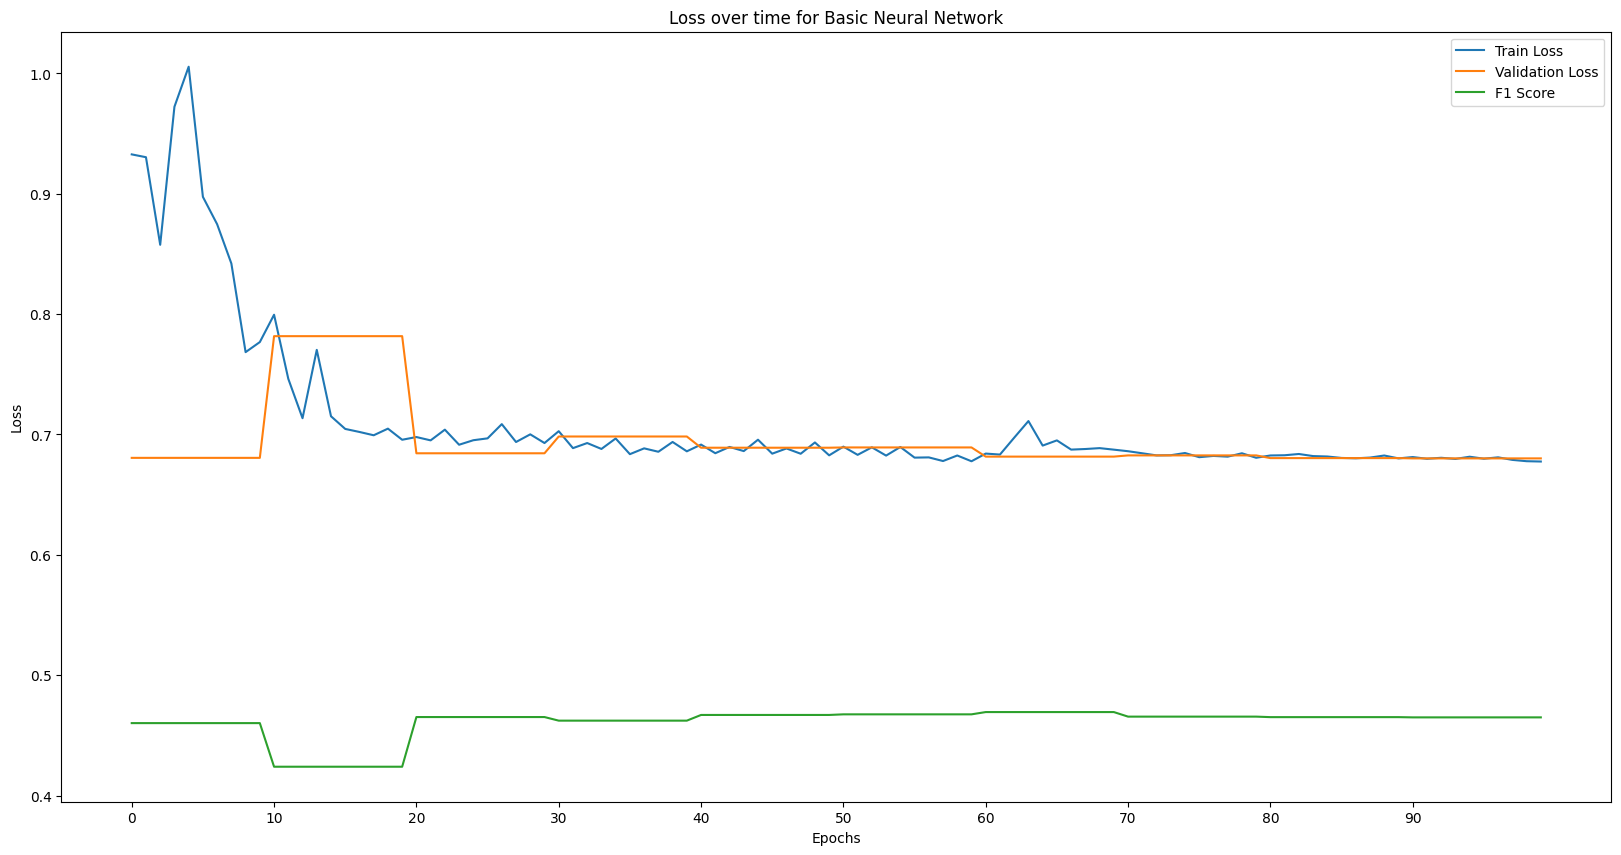
\includegraphics[width=0.8\textwidth]{results/nn_loss_overtime.png}
    \caption{This is a sample caption for the image.}
    \label{fig:sample-image}
 \end{figure}


\end{document}
